\documentclass[a4paper]{article}

\renewcommand{\labelenumii}{\theenumii}
\renewcommand{\theenumii}{\theenumi.\arabic{enumii}.}

\usepackage{fullpage} % Package to use full page
\usepackage{parskip} % Package to tweak paragraph skipping
\usepackage{tikz} % Package for drawing
\usepackage{amsmath}
\usepackage{amssymb,amsthm}
\usepackage{mathtools}
\usepackage{hyperref}
\usepackage{enumitem}
\usepackage{mathtools}
\usepackage{empheq}
\usepackage{amsfonts}
\usepackage{gensymb}
\usepackage{float}
\usepackage{subcaption}
\usepackage{placeins}


\newcommand*\widefbox[1]{\fbox{\hspace{2em}#1\hspace{2em}}}
%======================================== Title===========================================
\newcommand{\horrule}[1]{\rule{\linewidth}{#1}} 	% Horizontal rule
\title{
		\vspace{-0.6in} 	
		\usefont{OT1}{bch}{b}{n}
		\normalfont \normalsize \textsc{University of California Santa Cruz} \\ [10pt]
		\horrule{0.5pt} \\[0.4cm]
		\huge CMPE264 Proyect 1: High Dynamic Range (HDR) System \\
		\horrule{2pt} \\[0.5cm]
}
\author{
		\normalfont 								
        Aaron Hunter\\  Carlos Espinosa\\[-3pt]		\normalsize
        November 14, 2018
}
\date{}
%====================================Begin document=======================================
\begin{document}
\maketitle
%-----------------------------------------------------------------------------------------
\section*{Introduction}
This report documents a manual approach to creating a high dynamic range, or HDR, photograph.  HDR is a technique used to display  high contrast images by combining a series of two or more photos  at different exposure values taken of the same scene in order to boost the signal to noise ratio, or SNR, of the entire image.  Since most monitors can't project HDR images, the images are compressed using a tone mapping function which attempts to compress the contrast in a way that allows all areas of the image to retain significant detail, in other words it reduces the overall contrast ratio of the image, while preserving the relative values. \\

First we sought out a scene that would demonstrate the technique effectively.  Our initial thoughts were to get images during the daytime of the interior of a church with colorful stained glass windows receiving sunlight.  The challenge then would be to allow the very bright window to be displayed alongside interior details of the building and have both be clearly visible.  The state of religion being what it is, however, all the churches we visited on an early Saturday morning were locked.  There is one chapel, however, that is maintained as an historic site by the Holy Cross Church.  It is known as the Mission Chapel and dates back to the mid 1700's when Spain occupied the central coast of California.  This chapel turned out to be an ideal subject, at least from the technical standpoint.  Although it doesn't have the colorful stained glass we were seeking, we realized after looking at images on our camera that there was a faint cross made by the individual panes of glass in each window.  The effect is so faint that we didn't notice it at first.  The interior of the chapel is dimly lit with small incandescent lights mounted in a heavy iron candelabra. On the walls are old religious paintings that were difficult to see with the naked eye, much less photograph well.  Thus we found our challenge.  Create an image of the interior that contains both a directly sunlit window and a dark religious painting that allows the details of both to be seen. 

The following sections will detail our approach to generating the algorithm for creating an HDR image.  The first section deals with identifying the compression scheme that our camera uses when generating a JPEG file.  Although the camera is capable of producing ``raw'' images, that is, images that are linear over the entire range of the sensor, this first section attempts to invert the non-linear process used in the generation of  a JPEG file.  The second section shows each of the images collected for our project.  We will select three images from the collection and generate a linear version of each. In the third section we generate two different composite images, one which simply selects non-saturated pixels based upon their exposure, in other words, it combines the images based upon their SNR within the  scene.  We then create a second composite image using an average of the non-saturated pixels.  Finally, we use the built in Matlab tone mapping function to generate a compressed image for display on a standard monitor. 
%-----------------------------------------------------------------------------------------S1
\section{Camera Radiometric Calibration}
In preparation for this report we evaluated two cameras: a Sony Rx100 and  Fujifilm X-E1.  The compression scheme for the X-E1 appeared to be a smoother function so we chose that camera for the project.  Initially we took images in daylight at a gain value of ISO 200.  However, the pictures in the chapel required a higher gain for us to be able to take images over a broad range of exposure values, so we repeated the process at ISO 800.  The target image is a piece of standard printer paper, backed by a piece of white cardboard. We added the backer to minimize the transparency of the paper.  We took photos of the target in shade using a tripod at a range of exposure times from 1/60 sec to 1/4000 sec at f8 with the white balance set to daylight. We cropped a $100 \times 100$ pixel area of the picture and averaged over the cropped image to measure its average color.  The cropped images are presented in fig(\ref{fig:white}). 


 If a camera does not use a compression scheme for its JPEG image processing, a plot of the average color against  the exposure time will be linear.  For our camera, however, there is a strong non-linearity as seen in fig(\ref{fig:Ecal}).   What is notable about this camera is that the three colors behave very similarly and that the values are very close to one another depending on which portion of the original image we chose.  We tried two different methods for linearization, a polynomial fit and a power fit.  Although a cubic polynomial fits the data perfectly, between the data points the fit is suspect, so we chose a power law fit instead.  Its poor fit is at least repeatable between the color channels. The fitting parameters found for the exponential term for each channel are shown in table (\ref{tbl:gvals}). To determine these values we used the Matlab \verb+lsqcurvefit+ function specifying a fit to the data of the form $B' = g_0 * B^ {1/g}$, where $ B'$ is the recorded brightness of a given pixel, $ B$ is the actual value measured by the sensor,  $g_0$ and $g$  are the fitting parameters. This is a standard least squares fit that minimizes the residual between the data and the prediction.  Because we only care about the non-linear factor, we can safely ignore the proportionality constant when calculating the linear image values. 

\begin{table}[H]
    \begin{center}
        \begin{tabular}{l | c}
            Color & g\\
            \hline
            Red & 2.4678\\
            Green & 2.5483 \\
            Blue & 2.4473
    	\end{tabular}
    	\caption{Exponential fit parameter $g$ for each channel of the Fujifilm X-E1 camera}
    	\label{tbl:gvals}
    \end{center}
\end{table}

The fit of the data for each channel is shown in fig(\ref{fig:powerfit}.  It is clear that the linearization is not perfect, particularly for high brightness values. If we reverse the linearization process we obtain the approximately linear data shown in fig(\ref{fig:linEx}.  Although still retaining a convex shape the curvature relative to the recorded brightness values, $B'$ is reduced. 
\begin{figure}[htb!]
    \begin{center}
        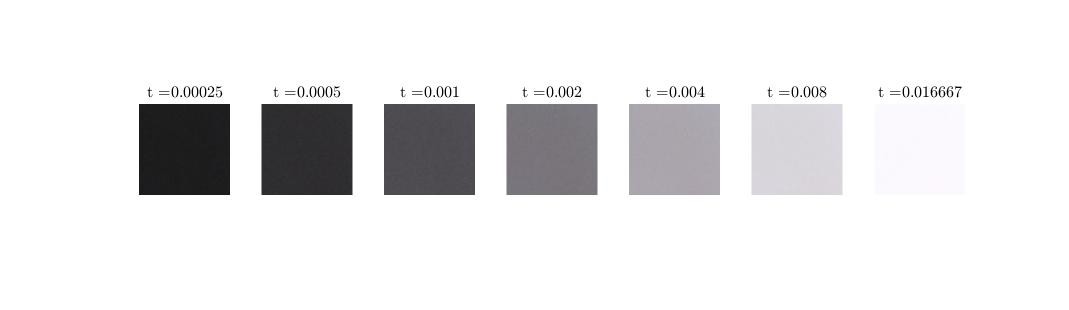
\includegraphics[width=\textwidth]{white_fuji.jpg}
	 \end{center}
    \caption{Fujifilm X-E1 white calibration images and exposure time. All images taken at ISO 800. These data span $67 \times$ exposure range} 
    \label{fig:white}
\end{figure}

\begin{figure}[htb!]
    \begin{center}
        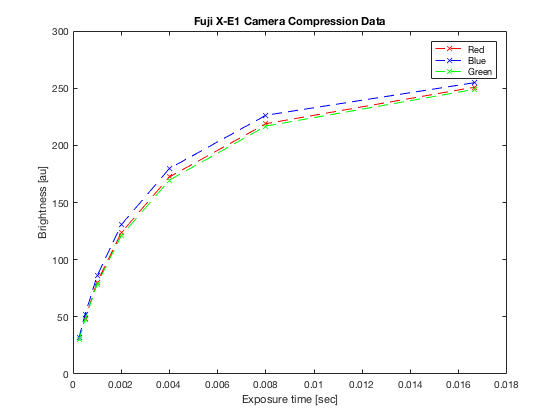
\includegraphics[width=4 in]{powerfit.png}
	 \end{center}
    \caption{Fujifilm X-E1 brightness values versus exposure time at ISO 800.} 
    \label{fig:Ecal}
\end{figure}


\begin{figure}[htb!]
    \begin{center}
        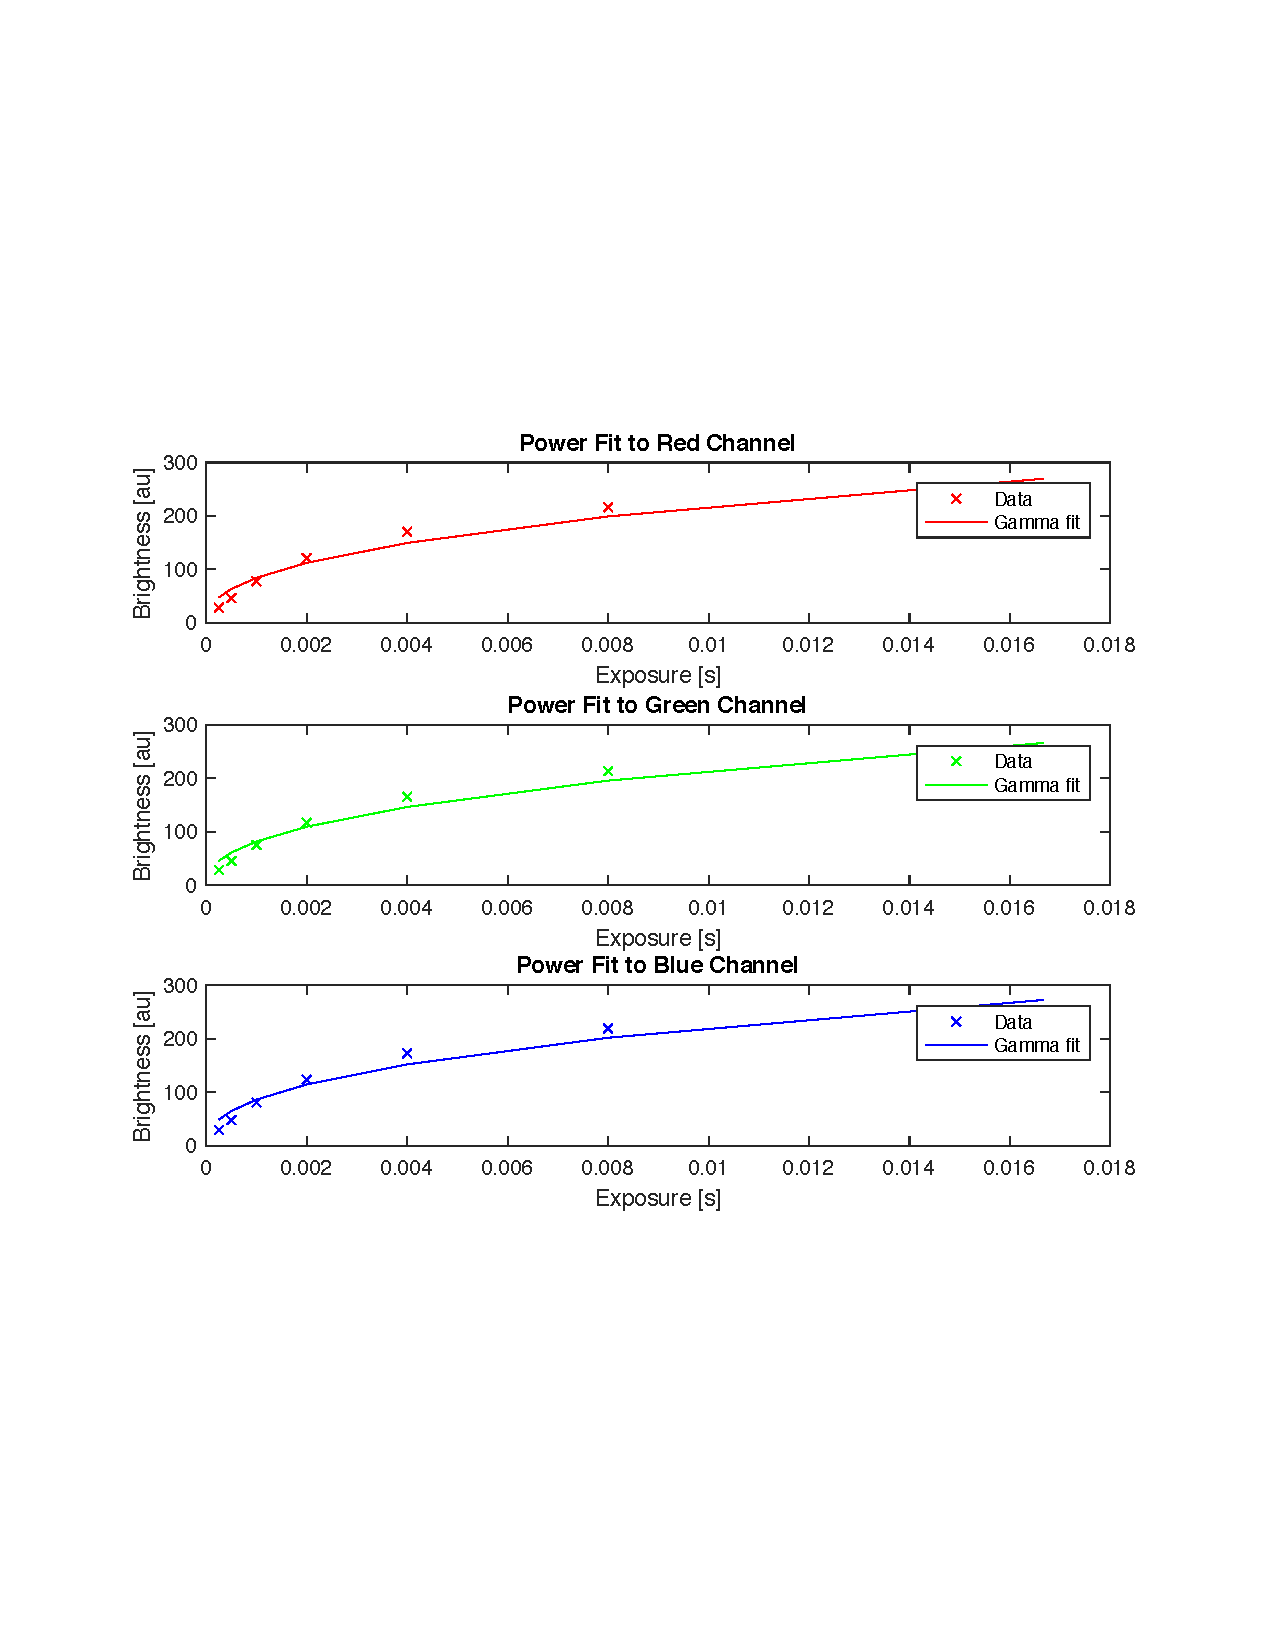
\includegraphics[width=4 in]{powerfit.pdf}
	 \end{center}
    \caption{Power fit to the exposure data for each color channel} 
    \label{fig:powerfit}
\end{figure}

\begin{figure}[htb!]
    \begin{center}
        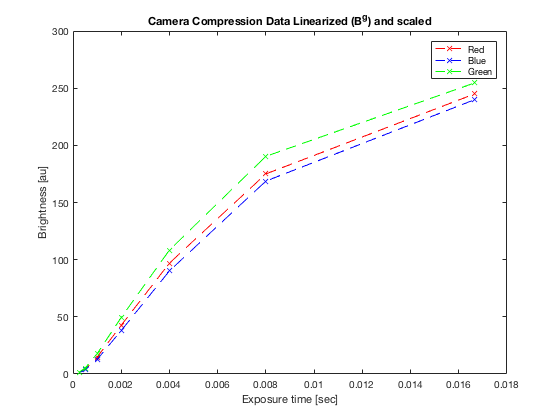
\includegraphics[width=5in]{linearExposure.png}
	 \end{center}
    \caption{Linearization results on exposure data for each channel.  Note that this fit to the camera data is not particularly good and the resulting linearization isn't particularly linear.  The important thing to
    note is that the response is more linear than the compressed data. } 
    \label{fig:linEx}
\end{figure}
\FloatBarrier
%---------------------------------------------
\section{Picture Stack Acquisition}
The photographs that we took inside the chapel are shown in fig(\ref{fig:stack}). In them the completely black areas demonstrate the pixels that are saturated and the histogram shows the brightness values once the saturated pixels are removed.  The darkest image is exposed such that the cross in the window is visible and not saturated.  It is taken at ISO 800 at 1/1000 of a second.  Each subsequent photograph is taken at twice the time of the previous one, up to the brightest photo in the collection taken at 1/60 second. To determine which images to use for our composite image, we evaluated each for their content.  The first picture selected is the one with no saturated pixels and clearly shows the faint cross made by the window panes.  The brightest image is also selected because it is exposed properly for the interior.  For the middle image we chose the one taken at 1/125 second because of the detail seen in the window sill itself. 

Fig(\ref{fig:imStack}) shows the three images selected with their respective histograms after linearization but before dividing by exposure ratio.

Fig(\ref{fig:hist1}) shows the  histograms for each color channel of the linearized photographs.  Fig(\ref{fig:hist2}) shows the histograms for the second and third images chosen once their overall brightness is reduced by the ratio of their exposure time versus the base image exposure time. 

\begin{figure}[H]
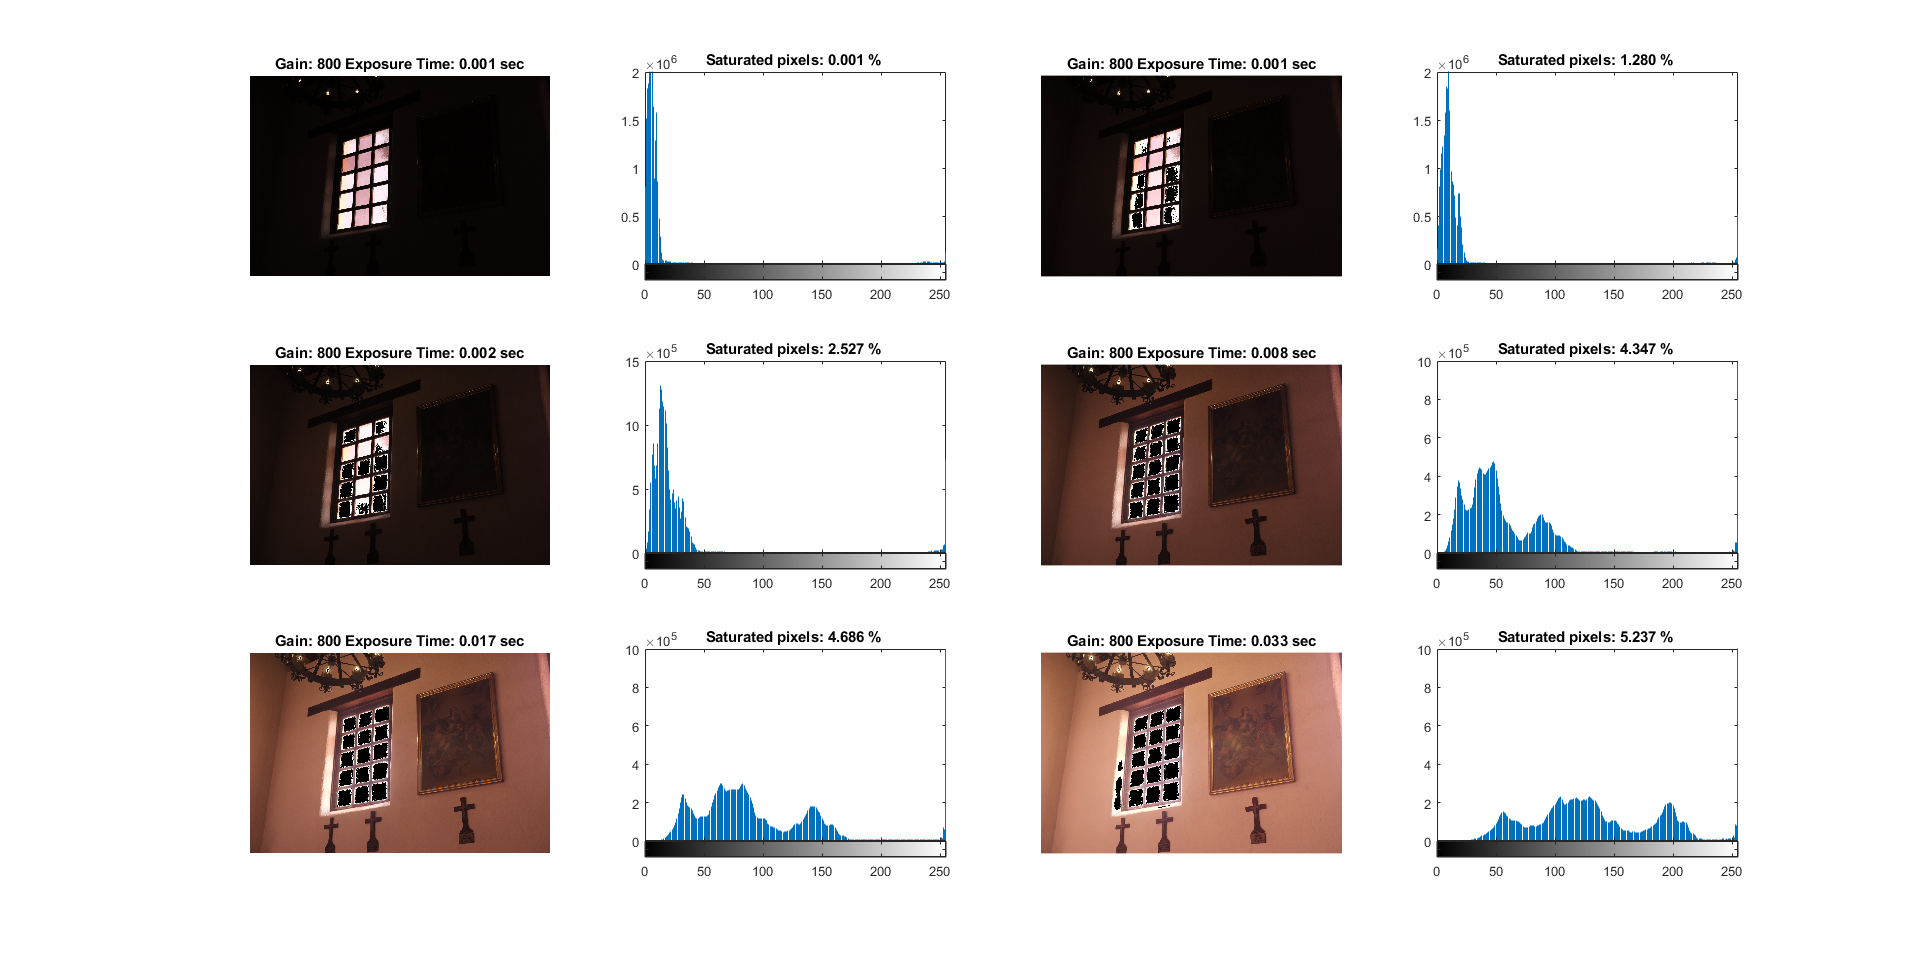
\includegraphics[trim=7cm 1cm 1cm 0cm clip, scale=.4]{Chapel_Histogram_set.png}
\caption{Picture Stack with ISO gain fixed at $G = 800$.  The first picture selected is the top left image.  The second is the middle right, and the third is bottom right.}
\label{fig:stack}
\end{figure}

\begin{figure}[htb!]
        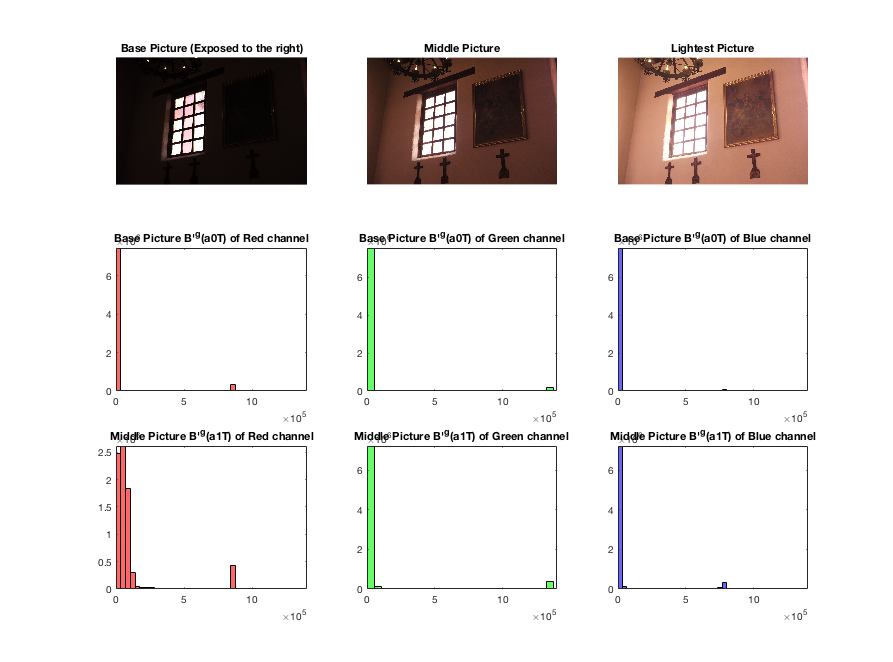
\includegraphics[width=\textwidth]{imStack.png}
    \caption{Image stack used for the HDR image and histograms} 
    \label{fig:imStack}
\end{figure}
\begin{figure}[htb!]
        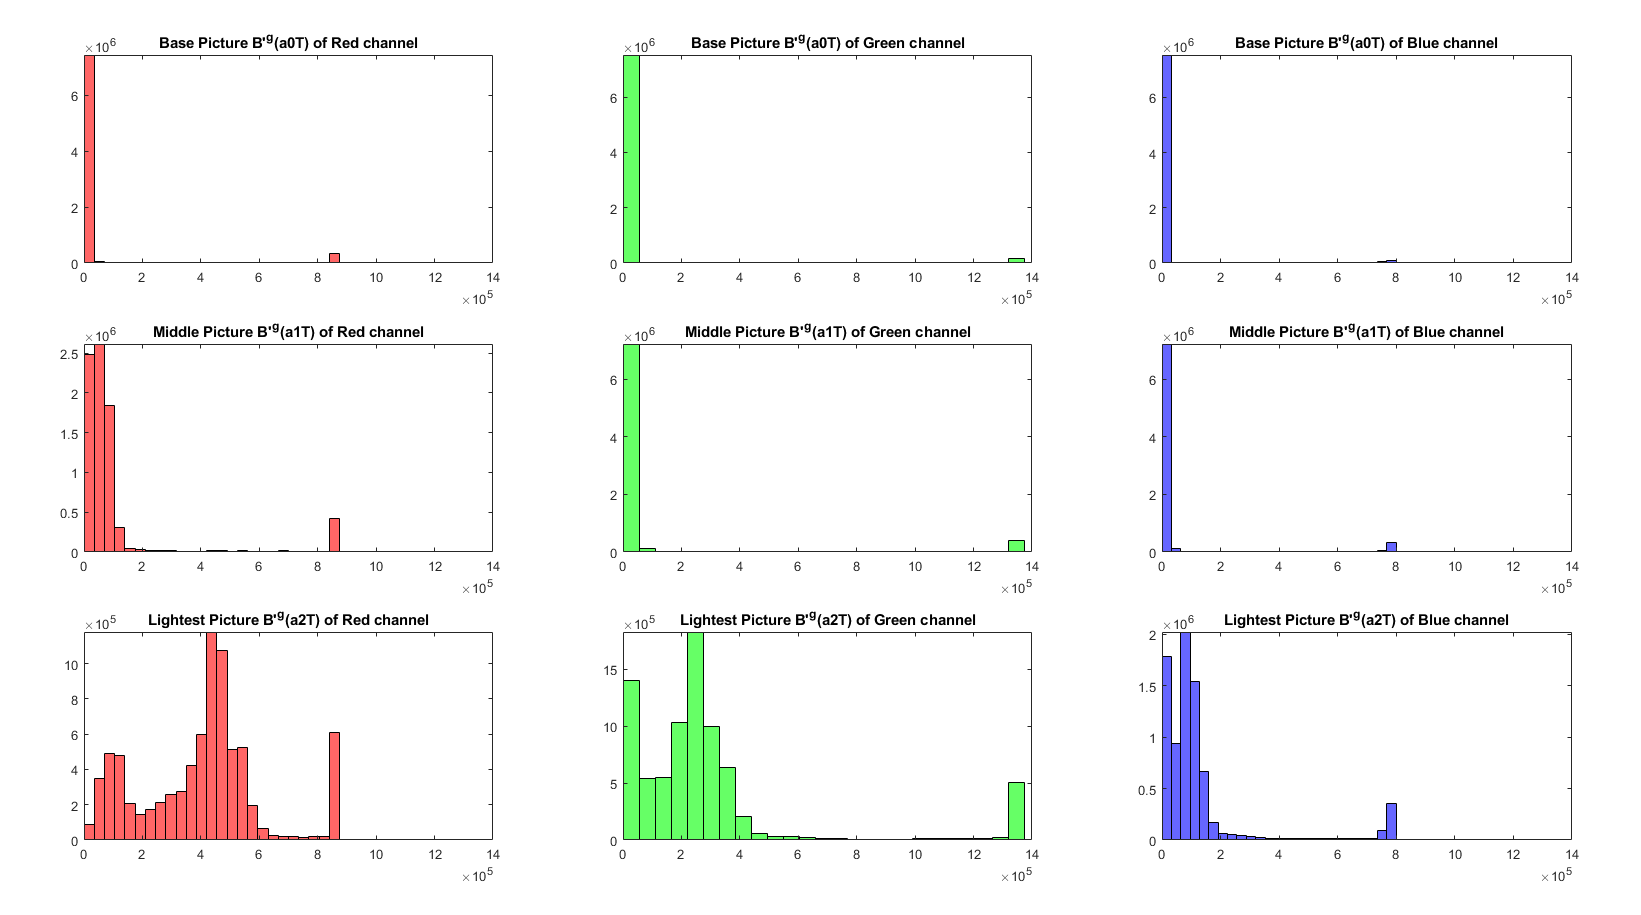
\includegraphics[width=\textwidth]{HistogramsLinearizedImages25Bins.png}
    \caption{Histograms for the linearized images} 
    \label{fig:hist1}
\end{figure}

\begin{figure}[htb!]
    \begin{center}
        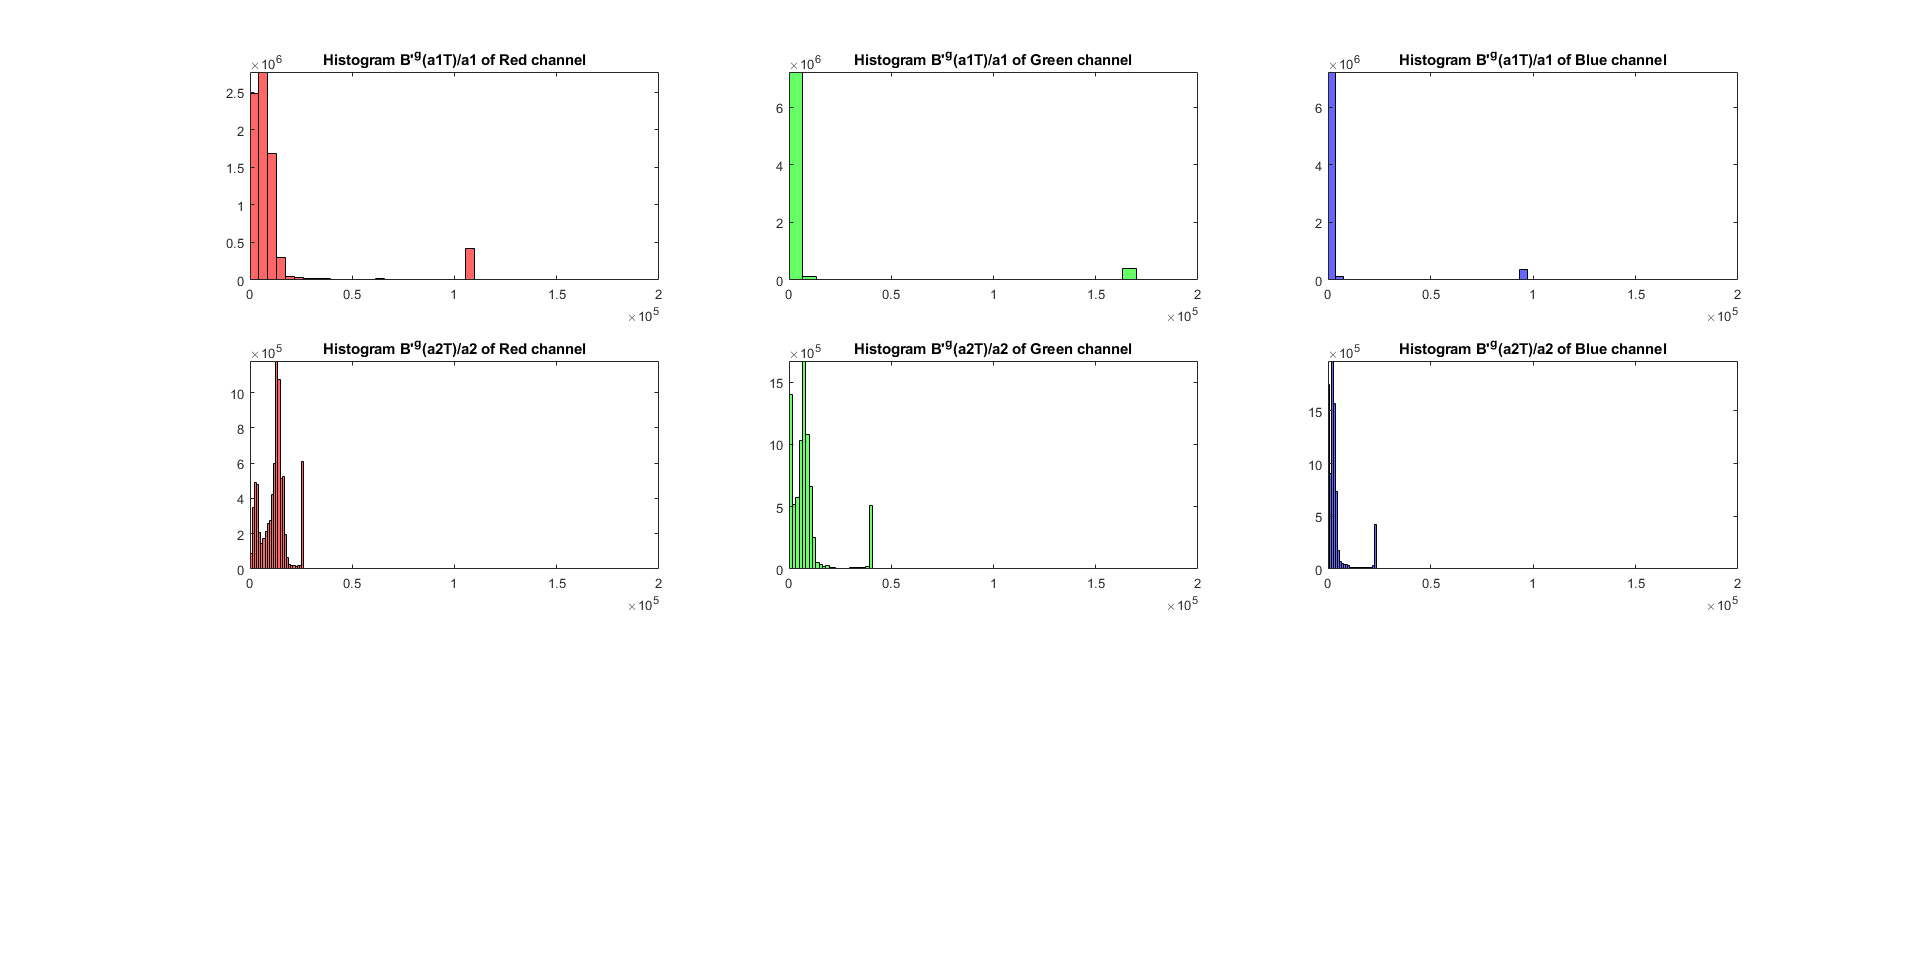
\includegraphics[width=\textwidth]{HistogramsScaledImages25Bins_RangeModified.png}
	 \end{center}
    \caption{Histograms for the linearized images, adjusted for exposure times.  Image 2 brightness values have been divided by $a_1 = 8$ and image 3 values have been divided by $a_2 = 33$} 
    \label{fig:hist2}
\end{figure}


\FloatBarrier
%-----------------------------------------------------------------------------------------S2
\section{Composite Image Creation}
In this section we explore two different methods for combing the linearized images selected in the previous section. .   The first method selects the pixels with the highest SNR between the three images and uses them for the composite image.  The second one doesn't throw away the non-saturated pixels.  Instead it takes the average of the pixels from the three images with non-saturated pixels. 

\subsection{Composite Algorithm 1}
 In the first composite image, we selected the pixels from image 1 where the brightness $B \ge E_{max} /a_1$ where $a_1 = 1000/125 = 8$ and $E_{max}$ is the brightest value in image 1. We do this by creating a mask of that allows all the values at the correct brightness and multiplying it to image 1.  We do this because we know that every pixel in image 2 (and image 3) in this region will be saturated.  We then create a mask from image 1 where $B  <E_{max} /a_2$ this mask is applied to image 3 pixels  divided by $a_2$ and represents the pixels with the highest SNR in this portion of the image.  Finally, we take the inverse of the two masks and generate the middle mask by multiplying them together.  This mask is then multiplied with image 2 pixels from this region divided by $a_1$ and represents the pixels with the highest SNR between $E_{max}/a_{2}$ and $E_{max}/a_1$.  The composite image is just the sum of the individual masked images.  The historgram for composite image 1 is shown in fig(\ref{fig:comp1}). The algorithm for the code generation is shown below for clarity.
 \begin{verbatim}
 ...
 mask = im1>= E_max/a(2);
mask1 = mask;
...
%mask the lowest exposure pixels
mask = im1 < E_max/a(3);
mask3 = mask;
...
%mask two is the inverse of mask1 and mask3
mask2 = not(mask1) .* not(mask3);
...
 \end{verbatim}

\FloatBarrier
\subsection{Composite Algorithm 2}
For the second composite image we take an average of the non-saturated pixels in a given region.  Clearly, the values from image 1 above $E_{max}/a_1$ can only come from image 1.  For the pixels that fall between  $E_{max}/a_{2}$ and $E_{max}/a_1$ we take the average of the pixels from image 1 and image 2.  For the remaining pixels the average of all three images is taken and applied.  The code for this is demonstrated in the following snippet.

 \begin{verbatim}
 ...
mask = im1>= E_max/a(2);
mask1 = mask;

mask = im1 < E_max/a(3);
mask3 = mask;

mask2 = not(mask1) .* not(mask3);

Image1 = (im1.*mask1);
Image2 = (im1.*mask2 + im2.*mask2/a(2))/2;
Image3 = (im1.*mask3 + (im2.*mask3)/a(2) +(im3.*mask3)/a(3))/3;
...
 \end{verbatim}

%-----------------------------------------------------------------------------------------S3
\section{Composite Image Reproduction}
Now that we have the HDR images we need a way to represent them.  If we naively convert them to 8 bit images we lose all the extra information that we added with the longer exposures.  For this report we used the tone map function within Matlab to generate standard resolution images.  Tone map functions by compressing the contrast of the scene while preserving the relative brightness values. Our initial attempts using the default parameters of the function resulted in a rather gray and flat image.  We adjust the saturation parameters to increase the intensity of the color and adjusted the lightness of the image to increase slightly the contrast.  The composite images are shown below.  Fig(\ref{fig:LDR1} is generated is the result using algorithm 1 above.  Fig(\ref{fig:LDR2}) is the image generated using the same parameters for tone map as used for composite image 1.  

The immediate thing to note about both images is that the cross made from the window is  visible despite the dramatic contrast of the real world scene.  Also the details in the painting are easily visible. This is actually quite remarkable because these details were difficult to see in person.  The differences between the images is subtle.  The second composite image has larger overall contrast despite using the same parameters to generate the tone map.  More importantly though, the detail around the window area is improved.  The color balance of both images is slightly off, perhaps due to the influence of the color of the incandescent lights located in the candelabra fixture.  
\begin{figure}[htb!]
    \begin{center}
        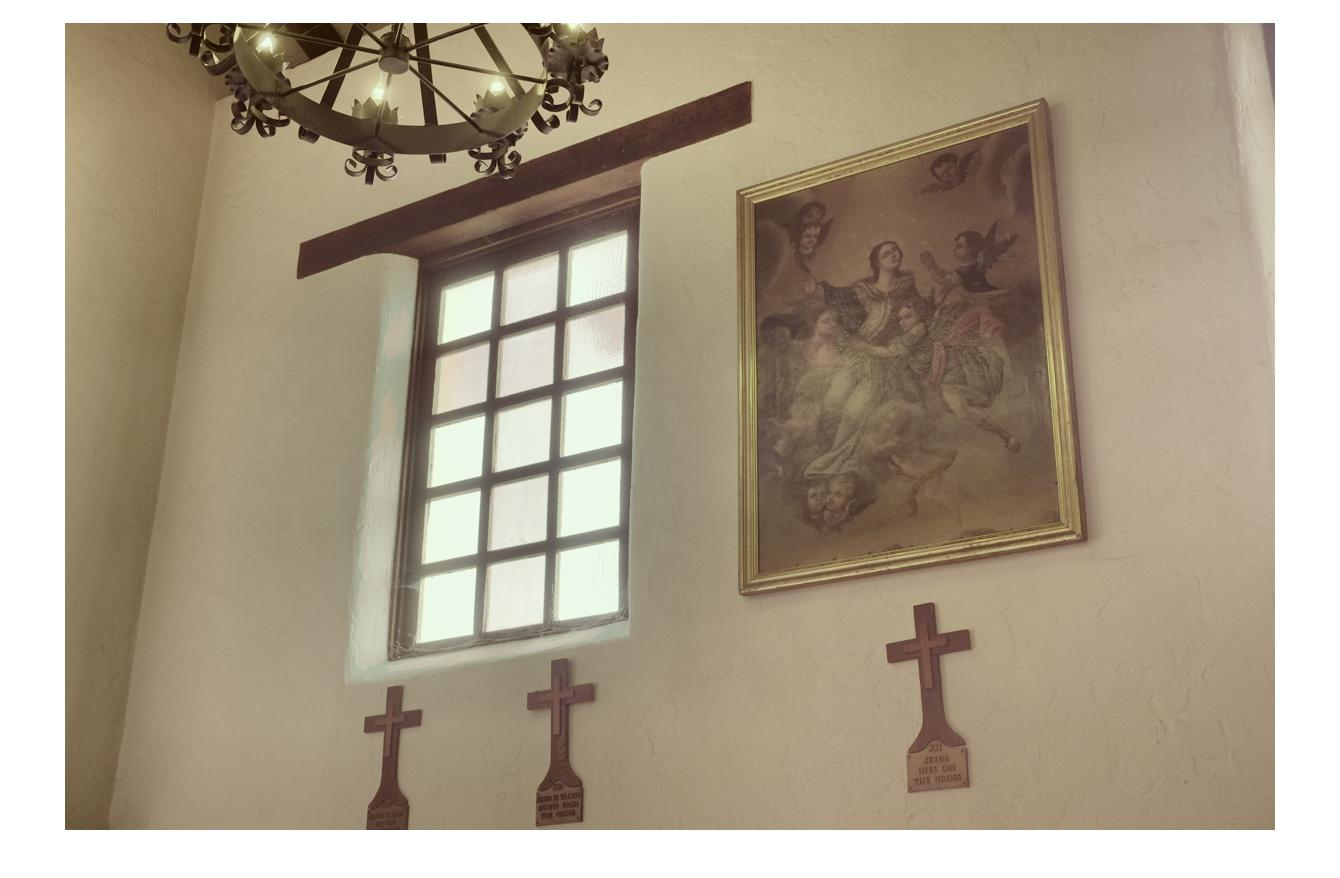
\includegraphics[width=6 in]{comp1LDR.jpg}
	 \end{center}
    \caption{Composite image 1 after tone map function} 
    \label{fig:LDR1}
\end{figure}

\begin{figure}[htb!]
    \begin{center}
        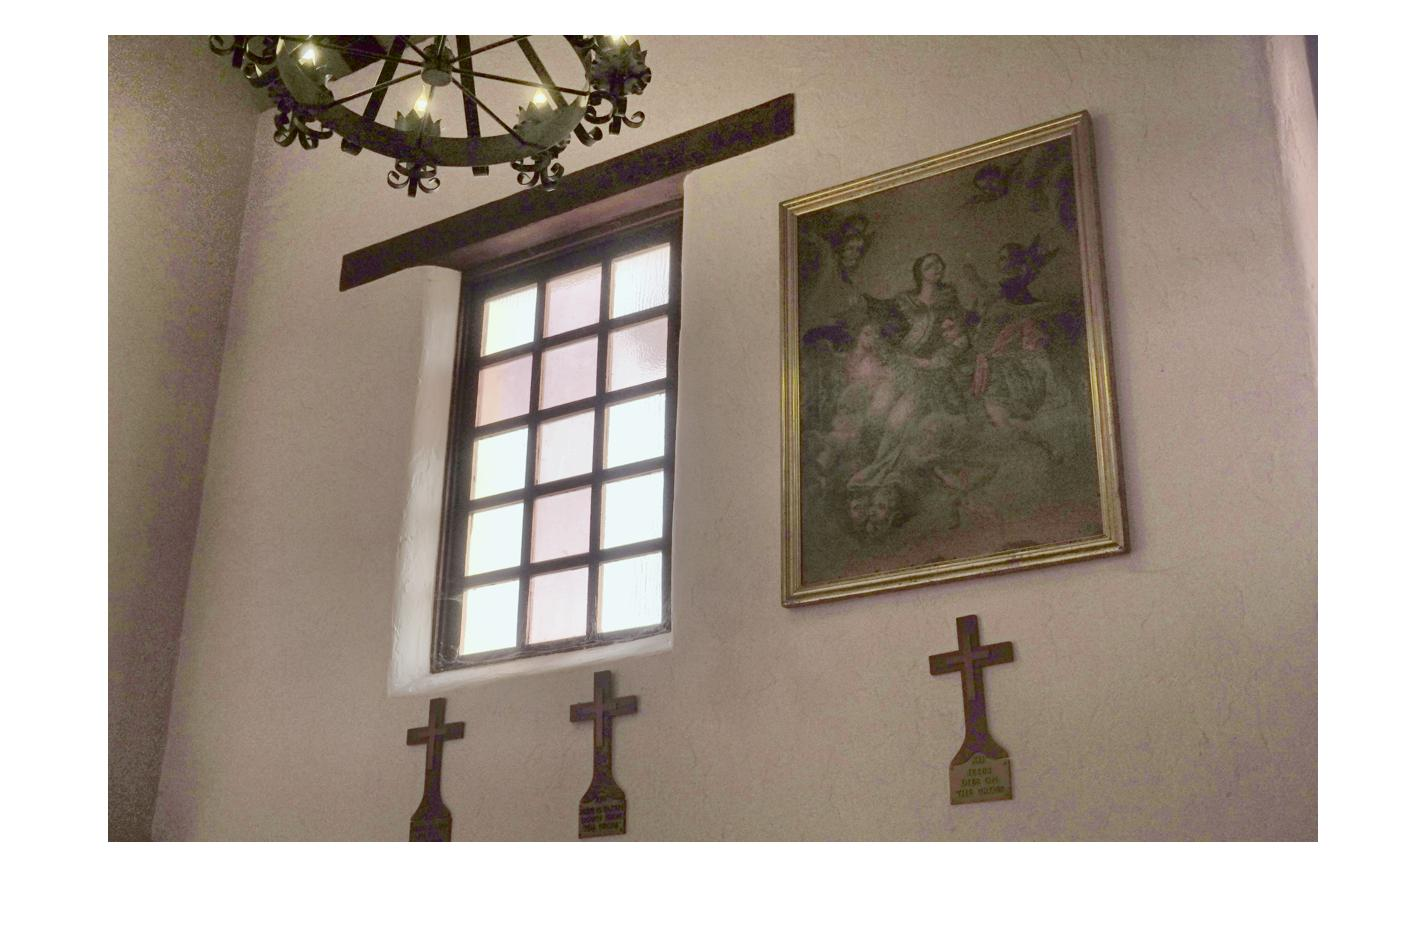
\includegraphics[width=6 in]{comp2LDR.jpg}
	 \end{center}
    \caption{Composite image 2 after tone map function} 
    \label{fig:LDR2}
\end{figure}
\FloatBarrier

\section{Conclusions}
In conclusion we have demonstrated the principle of generating HDR images by creating composite images from the same scene at multiple exposures.  The images we produced are ones that look realistic but actually do not exist in the real world.  In person the interior of the chapel was quite dark and the window was blinding.  The details of the painting were impossible to discern due to the bright window light. The slightly more sophisticated application demonstrated by the algorithm which uses all available information results in a visually more satisfying image, perhaps due to the greater amount of information encoded in the HDR image. More understanding of the tone map function would provide a better understanding of its output.  There are probably even more sophisticated ways to add all the picture information, perhaps weighting the pixels by their SNR.  

%%% End document
\end{document}